%%%%%%%%%%%%%%%%%%%%%%%%%%%%%%%%%%%%%%%%%%%%%%%%  import de package
\documentclass[12pt]{article}
\usepackage[utf8]{inputenc}
\usepackage[a4paper]{geometry}
\usepackage[myheadings]{fullpage}
\usepackage{lastpage}
\usepackage{setspace}
\usepackage{xcolor}
\usepackage{graphicx}
\usepackage{listings}
\usepackage{hyperref}
\usepackage{breakurl}

%%%%%%%%%%%%%%%%%%%%%%%%%%%%%%%%%%%%%%%%%%%%%%%%  ajout des lignes et zone de codes
\newcommand{\HRule}[1]{\rule{\linewidth}{#1}}
\onehalfspacing
\setcounter{tocdepth}{5}
\setcounter{secnumdepth}{5}
\definecolor{darkWhite}{rgb}{0.94,0.94,0.94}
\lstset{
  aboveskip=3mm,
  belowskip=-2mm,
  backgroundcolor=\color{darkWhite},
  basicstyle=\footnotesize,
  breakatwhitespace=false,
  breaklines=true,
  captionpos=b,
  commentstyle=\color{red},
  deletekeywords={...},
  escapeinside={\%*}{*)},
  extendedchars=true,
  framexleftmargin=16pt,
  framextopmargin=5pt,
  framexbottommargin=5pt,
  frame=tb,
  keepspaces=true,
  keywordstyle=\color{blue},
  language=Java,
  literate=
  {²}{{\textsuperscript{2}}}1
  {⁴}{{\textsuperscript{4}}}1
  {⁶}{{\textsuperscript{6}}}1
  {⁸}{{\textsuperscript{8}}}1
  {€}{{\euro{}}}1
  {é}{{\'e}}1
  {è}{{\`{e}}}1
  {ê}{{\^{e}}}1
  {ë}{{\¨{e}}}1
  {É}{{\'{E}}}1
  {Ê}{{\^{E}}}1
  {û}{{\^{u}}}1
  {ù}{{\`{u}}}1
  {â}{{\^{a}}}1
  {à}{{\`{a}}}1
  {á}{{\'{a}}}1
  {ã}{{\~{a}}}1
  {Á}{{\'{A}}}1
  {Â}{{\^{A}}}1
  {Ã}{{\~{A}}}1
  {ç}{{\c{c}}}1
  {Ç}{{\c{C}}}1
  {õ}{{\~{o}}}1
  {ó}{{\'{o}}}1
  {ô}{{\^{o}}}1
  {Õ}{{\~{O}}}1
  {Ó}{{\'{O}}}1
  {Ô}{{\^{O}}}1
  {î}{{\^{i}}}1
  {Î}{{\^{I}}}1
  {í}{{\'{i}}}1
  {Í}{{\~{Í}}}1,
  morekeywords={*,...},
  rulecolor=\color{black},
  showspaces=false,
  showstringspaces=false,
  showtabs=false,
  stepnumber=1,
  stringstyle=\color{gray},
  tabsize=4,
  title=\lstname,
}

%%%%%%%%%%%%%%%%%%%%%%%%%%%%%%%%%%%%%%%%%%%%%%%%%%%%  début du document %%%%%%%%%%%%%%%%%%%%%%%%%%%%%%%%%%%%%%%%%%%%%%%%
\begin{document}

%%%%%%%%%%%%%%%%%%%%%%%%%%%%%%%%%%%%%%%%%%%%%%%%  page de couverture
\begin{figure}[t]
	
\includegraphics[width=4cm]{logo_esiee.jpeg}
\end{figure}
\fontfamily{cmr} \selectfont
\title{ \normalsize \textsc{}
	\\ [2.0cm]
	\HRule{0.5pt} \\
	\LARGE \textbf{\uppercase{Rapport de projet d'Algorithmie}
	\HRule{2pt} \\ [0.5cm]
	\normalsize  \vspace*{5\baselineskip}}
}
\author{Théo PERESSE-GOURBIL et Manon HERMANN}
\date{Juin 2020}
\maketitle
\newpage

%%%%%%%%%%%%%%%%%%%%%%%%%%%%%%%%%%%%%%%%%%%%%%%%  table des matières
\tableofcontents
\newpage

%%%%%%%%%%%%%%%%%%%%%%%%%%%%%%%%%%%%%%%%%%%%%%%%  partie 1 du projet
\section{COCCINELLE ET PUCERONS}

%%%reponse aux questions-----------------------------------------------------------------------------------------------
\subsection{Réponse aux questions}
1) Lors de son périple, la coccinelle a mangé 279 pucerons. \newline
2) Son chemin sur la grille a été : (0,3)(1,2)(2,2)(3,1)(4,0)(5,0)(6,1)(7,0) \newline

%%%raisonnement--------------------------------------------------------------------------------------------------------
\subsection{Raisonnement}
Pour répondre au problème posé par la coccinelle, nous avions le choix parmi plusieurs algorithmes :
\begin{itemize}
    \item Un algorithme glouton qui ne répondrait pas forcément correctement aux attentes;

    \item Un algorithme qui explore TOUTES les possibilités et chemins. Cette solution n'est pas envisageable car le temps de calcul serait alors factoriel, ce qui avec de grands tableaux n'est pas viable,

    \item Un algorithme en programmation dynamique, ce qui était demandé. En effet, la programmation dynamique a pour but de passer par une matrice M(l,c), ce qui correspond assez bien a notre problème puisque nous avons justement un tableau 2D qui peut être vu comme une matrice.
\end{itemize}

Nous avons donc fait un programme en programmation dynamique. Nous avons calculé une matrice M(l,c) qui avait les propriétés suivantes : chaque case correspond au nombre maximal de pucerons que la coccinelle a mangé en arrivant sur cette case. De ce fait, appelons Grille le tableau contenant les pucerons et M la matrice.

Lors de l'initialisation, la première ligne de M est parfaitement égale à la première ligne de la grille, puisque la coccinelle n'aura pas bougé.

Ensuite, il faut avancer d'une case (l augmente de 1). Sachant que l'on ne peut se déplacer que vers le Nord, le Nord-est ou le Nord-Ouest, en choisissant la solution qui donne accès au plus de pucerons. \newline
On a donc :

\begin{lstlisting}
M[l][c] = grille[l][c] + max3(M[l-1][c-1],M[l-1][c],M[l-1][c+1])
\end{lstlisting}

\newpage
De proche en proche, on construit comme cela une matrice qui contient sur la dernière ligne le nombre total et maximal de pucerons que la coccinelle peut manger en arrivant sur cette case.
\newline Afin d'obtenir le nombre maximal de pucerons mangés, il suffit de trouver le maximum de la dernière ligne de la matrice.
\newline Pour connaître le chemin optimal, il faut parcourir la matrice M à l'envers. On part du plus grand de la dernière ligne, et on descend en allant soit au Sud, Sud-Est ou Sud-Ouest, tout en choisissant à chaque fois la case qui rapporte le plus de pucerons.
\newline Attention toutefois à ne pas sortir de la grille, il faut donc vérifier la position sur la grille en permanence.


%%%explication du code--------------------------------------------------------------------------------------------------
\subsection{Explication du code}
Dans cette section, nous expliquerons chaque fonction et son rôle, ainsi que des points sensibles de la fonction si besoin, dans l'ordre d'apparition dans le code source java.

\subsubsection{Main}
La fonction main est celle qui regroupe toutes les étapes du programme. En effet, elle sert juste à appeler correctement et dans l'ordre toutes les fonctions nécessaires dans l'algorithme, d'initialiser la grille de départ, gérer l'affichage des messages et mettre fin au programme.

\subsubsection{calculGrille}
Cette fonction permet la création de la matrice M selon la construction expliquée en 1.2. Nous initialisation une nouvelle matrice qui a la même taille que la grille, puis nous la remplissons, tout en faisant attention à ne pas dépasser.

\subsubsection{printGrille}
Cette fonction permet simplement d'afficher un tableau 2D.

\subsubsection{max3 et max2}
Ces deux fonctions similaires renvoient simplement le maximum de leur paramètres. Ces fonctions on été créées afin de ne pas surcharger le code avec des Math.max(x,Math.max(y,z));

\subsubsection{maxLigne}
Cette fonction calcule et revoie le maximum de la ligne passée en paramètre sous la forme d'un tableau à 2 cases : la première valeur correspond à la valeur maximum de la ligne et la seconde à son indice sur la ligne.
La fonction ajoute en bas de la liste les coordonnées de la plus grande case de la matrice, puis remonte et se remplit progressivement, jusqu'à arriver au haut. Au final, on obtient dans l'ordre le chemin avec chaque coordonnées.

\subsubsection{getTotal}
La fonction getTotal est simple et permet de renvoyer le maximum de pucerons mangés en appelant maxLigne.

\subsubsection{getPath}
Sûrement la fonction la plus compliquée du programme, cette fonction permet de retracer le chemin de la coccinelle. Cette fonction part de la fin de M et remplit un tableau 2D en commençant par la fin. Cette méthode peut sembler complexe à mettre en oeuvre, mais une fois bien programmée, elle permet d'accéder rapidement à n'importe quelle case de la matrice ou de la grille.

\subsubsection{getFirstCase et getLastCase}
Ces deux fonctions permettent d'obtenir les coordonnées de la première et de la dernière case sur laquelle la coccinelle s'est rendue.

\subsubsection{printCase et printPath}
Ces deux fonctions d'affichage servent juste à afficher ce qui leur est demandées.

\newpage


%%%%%%%%%%%%%%%%%%%%%%%%%%%%%%%%%%%%%%%%%%%%%%%%   partie 2 du projet
%%%redimensionnement d'images-------------------------------------------------------------------------------------------
\section{REDIMENSIONNEMENT D'IMAGES}
Le problème posé était le suivant : comment redimentionner des images sans perdre l'information importante et sans que l'image ne subisse de distorsions. En effet, si on "rogne" une image sur les bords ou aléatoirement, il y a un risque de perdre de l'information. De plus, la compression sans perte d'information entraîne souvent des distorsions sur l'image.
\newline Le but de ce programme est donc d'identifier les pixels importants, puis, grâce à la programmation dynamique, enlever les pixels les moins importants.

\subsection{Raisonnement pour la résolution de problème}
Le processus utilisé est celui du SeamCarving. Le SeamCarving se décompose en plusieurs étapes :
\begin{itemize}
    \item Calcul selon un critère choisis préalablement sur chaque pixel afin de déterminer les pixels les moins importants. Nous pouvons utiliser la densité, l'entropie, la luminosité... Pour ce programme, nous avons décidé d'utiliser la méthode de Sobel, qui consiste en le calcul du gradient de la luminosité de chaque pixel en fonction des pixels qui l'entoure. Cela permet de bien définir les contours car selon nous, le plus important dans une image sont les variations brusques de couleurs. En effet, une variation brusque (donc un gradient élevé) correspond généralement à un changement de surface sur une image, un changement de milieu. C'est ce changement qui contient toute l'information. Les critères cités ci-dessus ne nous satisfaisaient pas. En effet, si l'on prend l'exemple de la luminosité, et que l'on applique le SeamCarving sur une image disons blanche avec un motif complexe noir au centre, lors du calcul de la luminosité, le noir, qui a une valeur RGB de 0, sera alors tout de suite supprimé. Or l'information résidait dans le motif et non dans le fond blanc.

    \item Par la suite, il faut calculer des chemins à travers l'image ayant le plus faible coût. C'est ici que la programmation dynamique intervient. En effet, un chemin à travers une image correspond exactement à l'inverse du problème de la coccinelle. Nous voulons "manger" le moins possible ici. Il suffit ensuite de recomposer une nouvelle image avec une ligne ou une colonne en moins, puis de répéter l'opération autant de fois que nécessaire.
\end{itemize}
\newpage
Nous avons donc créer un constructeur qui dépend de l'état actuel de l'image. Ce constructeur a comme attributs des images et des valeurs. Les fonctions créées sont appelées sur cet objet, et ne concernent qu'une itération : enlever une ligne ou une colonne. Par la suite, dans les main, nous n'avons qu'à boucler le nombre voulu en créant à chaque fois un nouvel objet avec l'image créée par l'ancien constructeur, puis enlever une ligne ou une colonne.

La commande de compilation et d'exécution du programme est la suivante :
\begin{lstlisting}
$ javac SeamCarving.java
$ java SeamCarving "path_to_image" "%x" "%y"
\end{lstlisting}

%%%explication du code--------------------------------------------------------------------------------------------------
\subsection{Explication du code}
\subsubsection{Les classes importées}
Pour réaliser ce projet, nous avons eu besoin d'utiliser différentes classes, notament pour les images :
\begin{itemize}
    \item La classe \textit{BufferedImage} :
    Cette classe permet de récupérer des informations essentielles sur une image donnée comme la hauteur, la largeur, la valeur RGB de chaque pixel...

    \item La classe \textit{ImageIO} :
    La classe ImageIO permet d'ouvrir, de lire, et d'enregistrer des images au format BufferedImage. Elle fait le lien entre le type File (inputStream) et BufferedImage grâce à la méthode read.

    \item La classe \textit{File} :
    La classe File permet d'avoir accès à des inputStream, d'écrire et de lire des fichiers de tous types dans les fichiers de l'ordinateur. Cette classe nous a servi à ouvrir l'image souhaitée et à créer la nouvelle.

    \item La classe \textit{Math} :
    Math est une classe comportant des méthodes qui réalisent des opérations mathématiques. Nous nous en sommes servi dans les fonctions de minimum et de racine carré.
\end{itemize}
\newpage
\subsubsection{Les attributs}
Afin de réaliser notre algorithme, nous avons dans un premier temps créé une classe et un constructeur SeamCarving. Ce constructeur permettait d'initialiser facilement les attributs. Chaque objet de cette classe était principalement représenté par :
\begin{itemize}
    \item Deux attributs du type BufferedImage, une input, qui était l'image avant transformation, et une output qui était l'image après transformation;

    \item Deux entiers, width et height, qui représentaient respectivement la largeur et la hauteur de l'input, en pixel;

    \item Une matrice RGBimage qui correspond a une matrice de même taille que l'image d'entrée, dont chaque case correspond à la valeur au format RGB du pixel correspondant;

    \item Une matrice EnergyImage qui correspond à une matrice de même taille que l'image d'entrée, dont chaque case correspond à la valeur d'énergie du pixel correspondant, en suivant la méthode de Sobel, c'est à dire par le gradient.

    \item Deux matrices Mx et My, de même taille que l'image, dont chaque case correspond au minimum d'énergie parcouru en étant positionnée sur cette case. Mx a son minimum en haut et son maximum en bas, tandis que My a son minimum à gauche et son maximum à droite.

    \item Deux tableaux, pathX et pathY, à deux dimensions, correspondant au chemin le plus court, avec le moins d'énergie, parcourant la matrice Mx et My. La première case représente la coordonnée en x et la seconde en y.
\end{itemize}

\subsubsection{Constructeur \textit{SeamCarving}}
Le constructeur de la classe prend en paramètre une image de type BufferedImage et une chaîne de caractère. Il initialise tous les attributs. Le mode, représenté par la chaîne \textit{mode} permet de choisir entre 3 modes d'actions, afin de ne pas effectuer de calculs inutiles :
\begin{itemize}
    \item Le mode \textit{0}:
    Ce mode permet d'initialiser la première fois les attributs, sans effectuer de calculs;

    \item Le mode \textit{x}:
    Ce mode permet d'initialiser les attributs comme précédemment, mais en plus de lancer le calcul de Mx et pathX

    \item Le mode \textit{y}:
    Comme pour le mode \textit{x}, ce mode permet de lancer les calculs de My et pathY
\end{itemize}

Les différents modes permettent de gagner du temps sur les calculs. Lorsque l'on veut supprimer des pixels en x, inutile de calculer My et pathY, qui sont les deux fonctions les plus gourmandes en temps.

\subsubsection{getrgbImage}
Cette fonction permet d'obtenir la couleur en RGB de chaque pixel de l'image.
Elle transforme l'image d'entrée en une matrice rgbImage qui pourra ensuite être traitée dans le reste du code.

\subsubsection{getLuminance}
La fonction getLuminance permet d'obtenir un nombre représentant la quantité de luminance en chaque pixel. La fonction getRGB de la classe BufferedImage permet d'obtenir au format RGB la valeur RGB d'un pixel. Sous le format RGB, les 8 premiers bits sont pour le bleu, les 8 suivants pour le vert et les 8 derniers pour le rouge. \newline La formule suivante permet d'obtenir le niveau de gris correspondant :
\begin{lstlisting}
gris = (299*r + 587*g + 114*b)/1000;
\end{lstlisting}


\subsubsection{gradient}
Cette fonction utilise la méthode de Sobel. Pour chaque pixel, on regarde les pixels aux alentours (x+1, x-1, y+1,y-1) et on calcule la luminance de chacun d'entre eux grâce à la fonction getLuminance.
On calcul ensuite le gradient en x et en y, pour ensuite en calculer la norme.
Cette norme correspond au gradient du pixel(x,y) entré dans la fonction.

\subsubsection{setEnergy}
La fonction setEnergy permet d'éditer la matrice energyImage contenant le valeur du gradient pour chacun de ses pixels.
On utilisera par la suite cette matrice pour déterminer les pixels avec le moins d'importance.

\subsubsection{calculMx et calculMy}
Dans ces deux fonctions, on générera deux matrices Mx et My respectivement qui serviront à identifier le chemin de coût minimum en x et en y, afin de les retirer de l'image.

\subsubsection{getPathX et getPathY}
Les deux fonctions servent à calculer le chemin avec le coût le plus faible. Pour getPathX, on recherche l'énergie la plus petite de la dernière ligne. Puis on regarde, pour les pixels accessibles, celui qui est le plus petit. On parcours ainsi la matrice Mx de droite à gauche. Toutes les coordonnées sont entrées dans la variable pathX qui constitue le chemin de coût minimum. On fait de même dans getPathY, mais on parcours la matrice My de bas en haut.

\subsubsection{minColonne et minLigne}
Ces deux fonctions servent respectivement à calculer le minimum de la dernière colonne et le minimum de la dernière ligne. Ces deux fonctions servent au commencement de getPath.

\subsubsection{removeX et removeY}
Dans ces fonctions, on crée une nouvelle image que l'on va compléter sans les pixels appartenant à Path, cela revient à réduire de 1 la taille horizontale ou verticale de l'image d'origine. Pour ce faire, on recopie chaque pixel jusqu'à arriver à celui qu'il faut enlever, on saute ce pixel pour ensuite continuer à recopier les suivants décalé de 1.
La seule différence entre removeX et removeY est dans le sens de parcours des images.

\subsubsection{getPourcentage}
La fonction getPourcentage permet de convertir une chaîne de caractère saisie par l'utilisateur lors de l'exécution du programme en un Integer, tout en vérifiant le format.

\subsubsection{openImg}
Cette fonction sert de test pour ouvrir l'image au tout début du programme. Elle transforme un fichier, de type File, en une image exploitable par notre programme, de type BufferedImage.

\subsubsection{main}
La fonction main est celle qui regroupe toutes les étapes du programme. Elle vérifie tout d'abord que la commande est juste : il faut 3 arguments (nom de l'image, pourcentage de réduction horizontale, pourcentage de réduction verticale). Ensuite, elle sert juste à appeler correctement et dans l'ordre toutes les fonctions nécessaires dans l'algorithme. C'est aussi elle qui définie le nombre de fois que des lignes et colonnes doivent être supprimées pour obtenir la bonne réduction.


%%%problème rencontrés------------------------------------------------------------------------------------------------
\subsection{Problèmes rencontrés}

Lors de l'élaboration de ce projet, nous avons fait face à plusieurs problèmes :
\begin{itemize}
    \item Trouver le moyen d'éditer les images  \newline
    L'édition d'image était nouveau pour nous, nous avons donc du découvrir une nouvelle partie de Java, avec de nouvelles classes et fonctions. Nous avons mis un certain temps à parcourir la documentation officielle Oracle et trouver les fonctions dont nous avions besoin.

    \item Gradient de luminance : \newline
    Afin de trouver le bon paramètre, nous avons du chercher longtemps car comme nous l'expliquons plus haut, certains critères ne sont pas adaptés à cette méthode. La méthode de Sobel sur le gradient fonctionne particulièrement bien.

    \item Être cohérent entre x et y : \newline
    En informatique, le pixel de coordonnée (0,0) se situe en haut à gauche. De ce fait, il est compliqué de se représenter des tableaux inversés, la nomenclature devient alors très importante. Une erreur sur x ou sur y peut conduire à des résultats assez exotiques.
        \begin{figure}[h]
	        \begin{center} 
\includegraphics[width=3cm]{test.jpg}  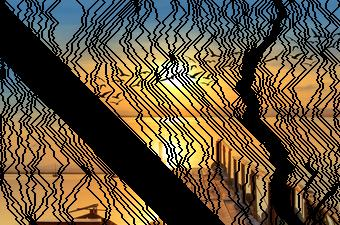
\includegraphics[width=5cm]{test2.jpg} \end{center}
	        \caption{cafouillage entre les coordonnées x et y}
        \end{figure}
    \newpage
    \item Raisonnement pour supprimer plusieurs fois une ligne/colonne : \newline
    Un problème s'est posé à la fin de notre projet. En effet, nous avions tout fait pour supprimer et identifier une ligne ou colonne à supprimer. Nous avons donc trouvé la solution : d'instancier l'objet le nombre de fois nécessaire et faire une boucle pseudo-récursive.
        \begin{figure}[h]
	        \begin{center} 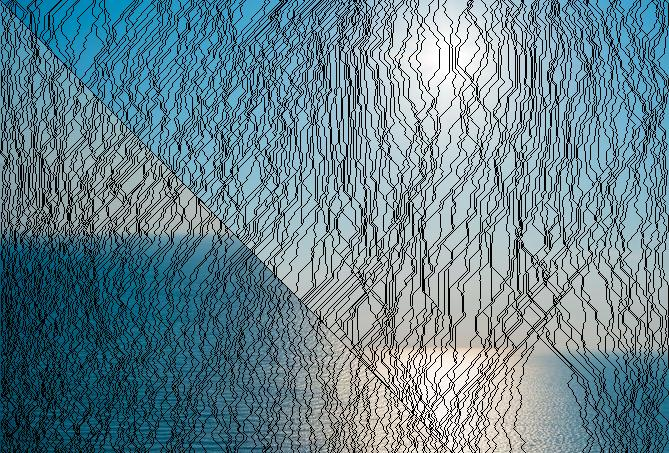
\includegraphics[width=6cm]{test3.jpg} \end{center}
	        \caption{problème décalage}
        \end{figure}
\end{itemize}

Afin d'éviter tout soucis au niveau organisation dans l'avancement du projet, plusieurs outils nous ont aidés :
\begin{itemize}
    \item Répertoire GitHub : \sloppy\burl{https://github.com/CappiLucky/Peresse_Hermann}
    \item Fonction télétype de Atom : pour pouvoir travailler en simultané sur le même document
    \item OverLeaf : Client LaTeX pour le rapport permettant de travailler en simultané sur le rapport
\end{itemize}

\newpage


%%%%%%%%%%%%%%%%%%%%%%%%%%%%%%%%%%%%%%%%%%%%%%%%  Sources
\section{Sources}
\begin{itemize}
    \item \sloppy\burl{https://www.developpez.net/forums/d418823/general-developpement/algorithme-mathematiques/contribuez/image-seam-carving/}

    \item \burl{https://fr.wikipedia.org/wiki/Seam\_carving}

    \item \sloppy\burl{https://docs.oracle.com/javase/7/docs/api/java/awt/image/BufferedImage.html}

    \item \sloppy\burl{https://docs.oracle.com/javase/7/docs/api/javax/imageio/ImageIO.html}

    \item \sloppy\burl{https://docs.oracle.com/javase/7/docs/api/java/io/File.html}

    \item \sloppy\burl{https://docs.oracle.com/javase/7/docs/api/java/lang/Math.html}

    \item \sloppy\burl{https://docs.oracle.com/javase/tutorial/2d/overview/images.html}

    \item \sloppy\burl{https://en.wikipedia.org/wiki/Sobel_operator}
\end{itemize}





\end{document}
